\documentclass[mathserif]{beamer}
\usepackage{amsmath}
\usepackage{graphicx}
\usepackage{multicol}
\usepackage{tikz}
\usetikzlibrary{decorations.pathreplacing}
\usetikzlibrary{arrows.meta, positioning, decorations.pathreplacing}

\title{Ultrafast and memory-efficient alignment of short DNA sequences
to the human genome}
\subtitle{\textit{Ben Langmead, Cole Trapnell, \\Mihai Pop and Steven L Salzberg}}

\author{Akshay Sanjeev}


\begin{document}
\begin{frame}
    \maketitle
\end{frame}

\section{Introduction}
\begin{frame}{We are in 2009}

\end{frame}

\begin{frame}{Outline of Bowtie}
    \begin{itemize}
        \item Burrows-Wheeler Transform(Indexing)
        \item Exact and inexact alignment
        \item Excessive backtracking
    \end{itemize}
\end{frame}

\section{Background}
\begin{frame}{Burrows- Wheeler Transform: Forward Transform}
    Let $T=\texttt{BANANA}$. BWT$(T)$ will be:
    \[
    \begin{bmatrix}
        \texttt{\$} &\texttt{B} &\texttt{A} &\texttt{N} &\texttt{A} &\texttt{N} &\texttt{A} \\
        \texttt{A} &\texttt{\$} &\texttt{B} &\texttt{A} &\texttt{N} &\texttt{A} &\texttt{N} \\
        \texttt{N} &\texttt{A} &\texttt{\$} &\texttt{B} &\texttt{A} &\texttt{N} &\texttt{A} \\
        \texttt{A} &\texttt{N} &\texttt{A} &\texttt{\$} &\texttt{B} &\texttt{A} &\texttt{N} \\
        \texttt{N} &\texttt{A} &\texttt{N} &\texttt{A} &\texttt{\$} &\texttt{B} &\texttt{A} \\
        \texttt{A} &\texttt{N} &\texttt{A} &\texttt{N} &\texttt{A} &\texttt{\$} &\texttt{B} \\
        \texttt{B} &\texttt{A} &\texttt{N} &\texttt{A} &\texttt{N} &\texttt{A} &\texttt{\$} \\
    \end{bmatrix} \pause 
    \rightarrow
    \begin{bmatrix}
        \texttt{\$} &\texttt{B} &\texttt{A} &\texttt{N} &\texttt{A} &\texttt{N} &\texttt{A} \\
        \texttt{A} &\texttt{\$} &\texttt{B} &\texttt{A} &\texttt{N} &\texttt{A} &\texttt{N} \\
        \texttt{A} &\texttt{N} &\texttt{A} &\texttt{\$} &\texttt{B} &\texttt{A} &\texttt{N} \\
        \texttt{A} &\texttt{N} &\texttt{A} &\texttt{N} &\texttt{A} &\texttt{\$} &\texttt{B} \\
        \texttt{B} &\texttt{A} &\texttt{N} &\texttt{A} &\texttt{N} &\texttt{A} &\texttt{\$} \\
        \texttt{N} &\texttt{A} &\texttt{\$} &\texttt{B} &\texttt{A} &\texttt{N} &\texttt{A} \\
        \texttt{N} &\texttt{A} &\texttt{N} &\texttt{A} &\texttt{\$} &\texttt{B} &\texttt{A} \\
    \end{bmatrix}\]
    \[
    BWT(T)\rightarrow \texttt{ANNB\$AA}
    \]

\end{frame}

\begin{frame}{BWT: Reverse Transform(UNPERMUTE)}
    \begin{center}
        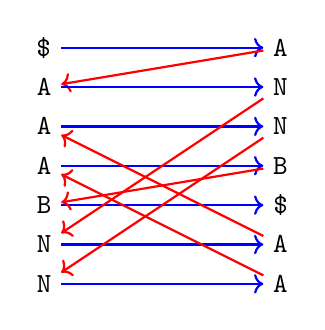
\begin{tikzpicture}
        % Horizontal distance = vertical height = 6 units
        \def\hsep{3}
        
        % Left column (top to bottom)
        \node (l1) at (0,3) {\texttt{\$}};
        \node (l2) at (0,2.5) {\texttt{A}};
        \node (l3) at (0,2) {\texttt{A}};
        \node (l4) at (0,1.5) {\texttt{A}};
        \node (l5) at (0,1) {\texttt{B}};
        \node (l6) at (0,.5) {\texttt{N}};
        \node (l7) at (0,0) {\texttt{N}};
        
        % Right column (top to bottom)
        \node (r1) at (\hsep,3) {\texttt{A}};
        \node (r2) at (\hsep,2.5) {\texttt{N}};
        \node (r3) at (\hsep,2) {\texttt{N}};
        \node (r4) at (\hsep,1.5) {\texttt{B}};
        \node (r5) at (\hsep,1) {\texttt{\$}};
        \node (r6) at (\hsep,.5) {\texttt{A}};
        \node (r7) at (\hsep,0) {\texttt{A}};
        \pause
        \draw[->, blue, thick] (l1) -- (r1);
        \pause 
        \draw[->, red, thick] (r1) -- (l2); % $ -> U
        \pause
        \draw[->, blue, thick] (l2) -- (r2); % 
        \pause
        % L-> R
        ; % 
        \draw[->, blue, thick] (l3) -- (r3); % 
        \draw[->, blue, thick] (l4) -- (r4); % 
        \draw[->, blue, thick] (l5) -- (r5); % 
        \draw[->, blue, thick] (l6) -- (r6); % 
        \draw[->, blue, thick] (l7) -- (r7); % 
        
        % Arrows from right to left (originally green, now blue)
        \draw[->, red, thick] (r2) -- (l6); % A -> V
        \draw[->, red, thick] (r3) -- (l7); % A -> $
        \draw[->, red, thick] (r4) -- (l5); % A -> B
        % \draw[->, red, thick] (r5) -- (l3); % B -> N
        \draw[->, red, thick] (r6) -- (l3); % N -> N
        \draw[->, red, thick] (r7) -- (l4); % N -> A

        \end{tikzpicture}
        \end{center}
    
        \pause
        \only<+->{\centering follow the tip of blue arrows to get back the initial message: \texttt{BANANA\$}}
    
\end{frame}

\begin{frame}{EXACTMATCH algoritham}
    $\Sigma=\texttt{B}_1\texttt{A}_1\texttt{N}_1\texttt{A}_2\texttt{N}_2\texttt{A}_3$.\\
    Pattern to find, $P = \texttt{NAN}$\\
    \begin{center}
        \begin{tikzpicture}
        % Horizontal distance = vertical height = 6 units
        \def\hsep{2}
        
        \node (l1) at (0,3) {\texttt{\$}};
        \node (l2) at (0,2.5) {\texttt{A}$_1$};
        \node (l3) at (0,2) {\texttt{A}$_2$};
        \node (l4) at (0,1.5) {\texttt{A}$_3$};
        \node (l5) at (0,1) {\texttt{B}$_1$};
        \node (l6) at (0,.5) {\texttt{N}$_1$};
        \node (l7) at (0,0) {\texttt{N}$_2$};
        % Right column (top to bottom)
        \node (r1) at (\hsep,3) {\texttt{A$_1$}};
        \node (r2) at (\hsep,2.5) {\texttt{N$_1$}};
        \node (r3) at (\hsep,2) {\texttt{N$_2$}};
        \node (r4) at (\hsep,1.5) {\texttt{B$_1$}};
        \node (r5) at (\hsep,1) {\texttt{\$}};
        \node (r6) at (\hsep,.5) {\texttt{A$_2$}};
        \node (r7) at (\hsep,0) {\texttt{A$_3$}};
        \pause
        %Indices:
        \node (il1) at (-1,3) {0};
        \node (il2) at (-1,2.5) {1};
        \node (il3) at (-1,2) {2};
        \node (il4) at (-1,1.5) {3};
        \node (il5) at (-1,1) {4};
        \node (il6) at (-1,.5) {5};
        \node (il7) at (-1,0) {6};

        %Right Indices
        \node (ir1) at (\hsep+1,3) {1};
        \node (ir2) at (\hsep+1,2.5) {5};
        \node (ir3) at (\hsep+1,2) {6};
        \node (ir4) at (\hsep+1,1.5) {4};
        \node (ir5) at (\hsep+1,1) {0};
        \node (ir6) at (\hsep+1,.5) {2};
        \node (ir7) at (\hsep+1,0) {3};
        \pause 
        \only<3>{\node[text=red] (top) at (-3, 3) {top$\rightarrow$};}
        \only<3>{\node[text=red] (bot) at (-3, 0) {bot$\rightarrow$};}

        \only<4>{\node[text=red] (top) at (-3, 0.5) {\texttt{N$_1$}$\rightarrow$};}
        \only<4>{\node[text=red] (bot) at (-3, 0) {\texttt{N$_2$}$\rightarrow$};}

        \only<5>{\node[text=red] (top) at (-3, 2) {\texttt{A$_2$N$_1$}$\rightarrow$};}
        \only<5>{\node[text=red] (bot) at (-3, 1.5) {\texttt{A$_3$N$_2$}$\rightarrow$};}
        
        \only<6>{\node[text=red] (top) at (-3, 0) {\texttt{N$_2$A$_2$N$_1$}$\rightarrow$};}
        \only<6>{\node[text=black] (bot) at (-3, 1) {\texttt{B$_1$A$_3$N$_2$}$\rightarrow$};}
        \end{tikzpicture}
    \end{center} 
\end{frame}

\section{Bowtie algorithm}
\begin{frame}{Exact vs Inexact matching}
    \begin{itemize}
        \item Exact matching performs poorly for DNA short read alignment because of mismatches from 
        sequencing errors and other reasons.
        \item New alignment algorithm which conducts a backtracking search to
        quickly find alignments that satisfy a specified alignment policy. 
        \item Each character in a read has a numeric quality value($m_i$), with
        lower values indicating a higher likelihood of a sequencing
        error. 
        \item We allows a limited number of mismatches, while trying to minimize $\sum_i m_i$, 
        where $i$ spans over all mismatches. 
    \end{itemize} 
    Bowtie is a quality-aware, greedy, randomized, depth-first search through the
    space of possible alignments.
\end{frame}

\begin{frame}{Excessive backtracking}
    If a particular suffix doesn't occur in the 
    text, the algorithm can backtrack. Backtracking involves \textbf{potentially substituting 
    a different base at an already-matched query position, introducing a mismatch, and 
    then resuming the search.}\\
\vspace{5mm}
    Excessive backtracking occurs when too many alternative paths are explored during the alignment 
    process due to mismatches. Bowtie uses double indexing to deal with this problem.
    Excessive backtracking is significant only when a read has many low-quality 
    positions and does not align or aligns poorly to the reference.
\end{frame}

\begin{frame}{Mismatch cases}
\begin{itemize}
    \item The high-quality base-pairs at 3' is called Seed(default: 28). 
    \item Seed is further divided into hi-half and lo-half each with 14bps.
    \item  Assuming the default mismatches(2), a reportable alignment can occur in 
    4 different ways. 
    \begin{enumerate}
        \item No mismatches in seed
        \item No mismatches in hi-half, one or two mismatches in lo-half
        \item No mismatches in lo-half, one or two mismatches in hi-half
        \item O ne mismatch in hi-half, one mismatch in lo-half
    \end{enumerate} 
\end{itemize}
\end{frame}

\begin{frame}{Phased Maq-like search}
    Bowtie uses a 3 phase approach:
    \begin{columns}
        \begin{column}{.3\textwidth}
        \begin{figure}
            \includegraphics[scale=.25]{media/fig3.png}
        \end{figure}
        \end{column}
        \begin{column}{.7\textwidth}
            \begin{enumerate}
            \item Phase 1 uses the mirror index and invokes the
            aligner to find alignments for cases 1 and 2. 
            \item Phases 2 and 3 cooperate to find alignments for case 3. Phase 2 finds partial
            alignments with mismatches only in the hi-half and phase 3
            attempts to extend those partial alignments into full align
            ments. Finally, phase 3 invokes the aligner to find alignments
            for case 4.
            \end{enumerate}
        \end{column}
    \end{columns}
\end{frame}

\section{Results}
\begin{frame}{Perfomance results}
\begin{figure}
    \includegraphics[width=\textwidth]{media/tab1.png}
\end{figure}
\pause
\begin{figure}
    \includegraphics[width=\textwidth]{media/tab2.png}
\end{figure}
\end{frame}

\begin{frame}{Perfomance Results-II}
    \begin{figure}
        \includegraphics[width=\textwidth]{media/tab3.png}
    \end{figure}
\end{frame}

\begin{frame}{Perfomance Results-III}
    \begin{figure}
        \includegraphics[width=\textwidth]{media/tab4.png}
    \end{figure}
    \pause
    \begin{figure}
        \includegraphics[width=\textwidth]{media/tab5.png}
    \end{figure}
\end{frame}

\begin{frame}{Summary}
    \begin{itemize}
        \item Bowtie's speed and small memory footprint are due chiefly to
        its use of the Burrows-Wheeler index in combination with the
        novel, quality-aware, backtracking algorithm introduced
        here. Double indexing is used to avoid the performance penalty
        of excessive backtracking.
        \item Bowtie exhibits a large performance advantage over both Maq
        and SOAP when mapping reads to the human genome.
        \item  Unlike many other short-read aligners, Bowtie creates a per
        manent index of the reference that may be re-used across
        alignment runs. 
    \end{itemize}
\end{frame}
\end{document}